\begin{frame}{Application 1}
\end{frame}
%--------------------------------------------------------------------------------------
\begin{frame}{The changing mobile landscape}
\begin{block}{}
\begin{itemize}
\item 5G will not only be ``4G but faster" but will support new models such as IoT
\item Current wireless - a few devices with sustained connectivity
\item Future wireless -  \alert{massive} no. of devices requesting \alert{sporadic} connectivity
\end{itemize}
\end{block}
\begin{center}
\includegraphics[width=4.5in]{C:/Users/nrkri/Dropbox/Work/RESEARCH/Projects/MACcollision/Figures/5Gchanginglandscape}
\end{center}
\end{frame}
%------------------------------------------------------------------------------------
\begin{frame}{The changing mobile landscape}
\begin{block}{}
\begin{itemize}
%\item 5G will not only be ``4G but faster" but will support new models such as IoT
\item Current wireless - a few devices with sustained connectivity
\item Future wireless -  \alert{many uncoordinated} devices requesting \alert{sporadic} connectivity
\end{itemize}
\end{block}
\begin{center}
\includegraphics[width=2.75in]{C:/Users/nrkri/Dropbox/Work/RESEARCH/Projects/MACcollision/Figures/machinetomachine}
\end{center}
\end{frame}
%------------------------------------------------------------------------------------
\begin{frame}{The changing mobile landscape}
\begin{block}{}
\begin{itemize}
%\item 5G will not only be ``4G but faster" but will support new models such as IoT
\item Current wireless - a few devices with sustained connectivity
\item Future wireless -  \alert{many uncoordinated} devices requesting \alert{sporadic} connectivity
\end{itemize}
\end{block}
\begin{center}
\includegraphics[width=2.75in]{C:/Users/nrkri/Dropbox/Work/RESEARCH/Projects/MACcollision/Figures/vehicular_sensor_networks}
\end{center}
\end{frame}
%------------------------------------------------------------------------------------
\begin{frame}{A possible MAC frame structure}
\begin{itemize}
\item Total of $Q$ users out of which $K$ are active
\item $Q$ is very large and $K$ is a small fraction of $Q$
\end{itemize}
\begin{figure}[t!]
  \begin{center}
  %\scalebox{0.85}{\input{../../Projects/MACcollision/Figures/slotstructurewithoutfb}}
\begin{center}
\includegraphics[width=4.5in]{C:/Users/nrkri/Dropbox/Work/RESEARCH/Projects/MACcollision/Figures/slotstructurewithoutfb}
\end{center}
%  \caption{At the onset of a frame, the base station heralds the start of a new round, and transmits a beacon for coarse synchronization. It then estimates the number of active devices, and subsequently broadcasts the number of slots contained within the frame. This header is followed by a sequence of time slots during which codewords are transmitted in a largely uncoordinated manner.}
%  \caption{Proposed structure: synchronization beacon, population estimation, slot sequence, \& feedback.}
%  \label{fig:framework}
  \end{center}
\end{figure}
\begin{itemize}
\item Beacon is used to obtain coarse synchronization
\item Each user transmits a signature sequence
\item BS estimates the no. of users ($K$) (Chen, Guo '14, Calderbank)
\item Picks an $M$ and broadcasts it
\end{itemize}
\end{frame}

%------------------------------------------------------------------------------------

\begin{frame}{System under consideration}
\begin{itemize}
\item Wireless network with \textcolor{blue}{$K$ distributed users} (no coordination)
\item Each user has one packet of info to transmit to a central receiver
\item Total \textcolor{red}{time is split into $M$ slots} (packet duration)
    \begin{itemize}
    \item Some policy used to decide if they transmit in $j$-th slot or not
    \item Receiver knows the set of users transmitting in the $j$-th slot
    \end{itemize}
\end{itemize}
\vspace*{-0.1in}
\begin{center}
\includegraphics[width=2.5in]{C:/Users/nrkri/Dropbox/Work/RESEARCH/Projects/MACcollision/Figures/systemmodel1}
\end{center}
\end{frame}

%------------------------------------------------------------------------------------
\begin{frame}{Random access paradigm}
\begin{itemize}
\item $k$-th user:
\begin{itemize}
  \item Generates a random variable $D_k \in \{1,\ldots,M\}$
  \item Generating PMF is $f_D$, i.e., \alert{$Pr(D_k=i) = f_D[i]$}
  \item Transmits during $D_k$ time slots drawn uniformly from $\{1,\ldots,M\}$
\end{itemize}
\end{itemize}
\begin{center}
\includegraphics[width=2.5in]{C:/Users/nrkri/Dropbox/Work/RESEARCH/Projects/MACcollision/Figures/systemmodel2}
\end{center}
\vspace{-3mm}
\begin{itemize}
\item In this example, $D_3 = 3$ and user 3 transmits in slots $\{1,3,5\}$
%\item Our setup is based on Liva 2011 \& Paolini et al. 2012
\end{itemize}
\end{frame}
%------------------------------------------------------------------------------------
\begin{frame}{Iterative interference cancelation}
\begin{itemize}
\item \textcolor{red}{If exactly one user transmits per slot, then packet is decoded w.h.p.}
\vspace{1mm}
\item \textcolor{blue}{If more than one user transmits per slot, then collision}
    \begin{itemize}
\vspace{1mm}
    \item Rx subtracts previously decoded packets from collided packets
\vspace{1mm}
    \item If Rx can subtract all but one, remaining packet is decoded w.h.p.
\vspace{1mm}
    \item Otherwise, the received packet is saved for future processing
\vspace{1mm}
    \item Once all $K$ packets recovered, an ACK terminates the transmission
\vspace{1mm}
    \item Similar to interference cancellation in multi-user detection
    \end{itemize}
\end{itemize}
\vspace*{-0.1in}
\begin{center}
\includegraphics[width=2.5in]{C:/Users/nrkri/Dropbox/Work/RESEARCH/Projects/MACcollision/Figures/iterativeinterferencecancellation2}
\end{center}
\end{frame}
%------------------------------------------------------------------------------------
\begin{frame}{Performance measure - Efficiency}
 \begin{itemize}
    \item Suppose \textcolor{red}{$M$ time slots} needed to successfully transmit all $K$ packets
\vspace{6mm}
    \item Then, the \textcolor{blue}{efficiency of the system} is said to be \[\eta = K/M \; \text{packets/slot} \]
 \end{itemize}
\end{frame}
%------------------------------------------------------------------------------------
\begin{frame}{Graphical representation (Liva 2012)}
\begin{itemize}
\item Tanner graph representation for the transmission scheme
\item Variable nodes $\leftrightarrow$ users, Check nodes $\leftrightarrow$ received packets
\item Message-passing decoder - \textcolor{blue}{peeling decoder} for the erasure channel
\end{itemize}
\begin{center}
\includegraphics[width=3.75in]{./Figures/iterativeinterferencecancellation2}
\end{center}
%\begin{minipage}[t]{0.48\linewidth}
%\begin{center}
%\includegraphics[width=1.75in]{../../Projects/MACcollision/Figures/graphicalmodel}
%\end{center}
%\end{minipage}
%\begin{minipage}[t]{0.48\linewidth}
%\begin{center}
%\includegraphics[width=1.75in]{../../Projects/MACcollision/Figures/graphicalmodelmsgpassing}
%\end{center}
%\end{minipage}
\pause
\begin{block}{}
\begin{itemize}
\item $L_i$ ($R_i$) - fraction of left (right) nodes with degree $i$ - notice that $\boxed{L_i = f_D[i]}$
\item $\lambda_i$ ($\rho_i$) - fraction of edges connected to left (right) nodes with deg $i$
\end{itemize}
\end{block}
\end{frame}
%%------------------------------------------------------------------------------------
\begin{frame}{Low density generator matrix (LDGM) codes}
\vspace{-3mm}
\begin{columns}
\begin{column}{0.47\textwidth}
\begin{center}
\includegraphics[width=2.0in]{./Figures/LDGM}
\end{center}
\end{column}
\begin{column}{0.47\textwidth}
\begin{itemize}
\item $L(x) = \frac14 x + \frac14 x^2 + \frac12 x^3$
\vspace{2mm}
\item $\lambda(x) = \frac19 + \frac29 x + \frac 69 x^2$
\vspace{2mm}
\item $R(x) = \frac15 x + \frac45 x^2$
\vspace{2mm}
\item $\rho(x) = \frac19 + \frac89 x$
\vspace{2mm}
\item Rate $R = \frac{\int_{0}^{1}\lambda(x) \ dx}{\int_{0}^{1} \rho(x) \ dx}$
\end{itemize}
\end{column}
\end{columns}

\begin{columns}
\column{0.45\textwidth}
\begin{block}{DE for LDPC}
\vspace*{-3mm}
\begin{eqnarray*}
  x_0 &=& \epsilon \\
  y_l &=& 1-\rho(1-x_{l-1}) \\
  x_l &=& \epsilon \lambda(y_l)\\
  x_l &=& \epsilon \lambda(1-\rho(1-x_{l-1}))
\end{eqnarray*}
\end{block}

\column{0.45\textwidth}
\begin{block}{DE for LDGM}
\vspace*{-3mm}
\begin{eqnarray*}
  x_0 &=& 1 \\
  y_l &=& 1-\rho(1-x_{l-1}) \\
  x_l &=& \lambda(y_l) \\
  x_l &=& \lambda(1-\rho(1-x_{l-1}))
\end{eqnarray*}
\end{block}
\end{columns}
\end{frame}
%%------------------------------------------------------------------------------------
%\begin{frame}{Analysis of the scheme - degree distributions}
%%\begin{block}{}
%%\begin{itemize}
%%\item $L_i$ ($R_i$) - no. of left (right) nodes with degree $i$
%%\item $\lambda_i$ ($\rho_i$) - no. of edges connected to left (right) nodes with deg $i$
%%\end{itemize}
%%\end{block}
%\begin{itemize}
%\item For a given $f_D$, the scheme results in an ensemble of LDGM codes
%\vspace{2mm}
%\begin{itemize}
%\item VN d.d. from node perspective - $L(x) = \sum_i L_i x^i$ ($L_i = f_D[i]$)
%\vspace{1mm}
%\item VN d.d. from edge perspective - $\lambda(x) = \sum_i \lambda_i x^{i-1} = \frac{L'(x)}{L'(1)}$
%\vspace{1mm}
%\item CN d.d. from node perspective - $R(x) = \sum_i R_i x^i$
%\vspace{1mm}
%\item CN d.d. from edge perspective - $\rho(x) =\sum_i \rho_i x^{i-1} = \frac{R'(x)}{R'(1)}$
%\end{itemize}
%\item ${\texttt{l}}_{avg} = L'(1)$ and ${\texttt{r}}_{avg} = \frac{K}{M} {\texttt{l}}_{avg}$
%\end{itemize}
%
%\begin{block}{Efficiency of the scheme}
%\[
%\eta = \frac{K}{M} = \frac{{\texttt r}_{avg}}{{\texttt l}_{avg}} =
%\frac{R'(1)}{L'(1)}
%\]
%\end{block}
%\end{frame}
%%------------------------------------------------------------------------------------
%\begin{frame}{Example of degree distributions}
%\begin{columns}
%\begin{column}{0.47\textwidth}
%\begin{center}
%\includegraphics[width=1.75in]{../Figures/graphicalmodel}
%\end{center}
%\end{column}
%\begin{column}{0.47\textwidth}
%\begin{itemize}
%\item $L(x) = \frac14 x + \frac14 x^2 + \frac12 x^3$
%\vspace{3mm}
%\item $\lambda(x) = \frac19 + \frac29 x + \frac 69 x^2$
%\vspace{3mm}
%\item $R(x) = \frac15 x + \frac45 x^2$
%\vspace{3mm}
%\item $\rho(x) = \frac19 + \frac89 x$
%\end{itemize}
%\end{column}
%\end{columns}
%\end{frame}
%------------------------------------------------------------------------------------
\begin{frame}{Poisson approximation for check node d.d.}

\vspace{-0.15in}
\begin{center}
\hspace{14mm} \includegraphics[width=2.0in]{C:/Users/nrkri/Dropbox/Work/RESEARCH/Projects/MACcollision/Figures/poissonapprox}
\end{center}
\vspace{-0.15in}
\begin{block}{Slot transmission probability}
User $k$ transmits in slot $m$ with prob. $p = \sum_{i=1}^\infty L_i \frac{i}{M} = \frac{\texttt{l}_{avg}}{M} = \frac{\texttt{r}_{avg}}{K}$ \pause
\end{block}
\begin{block}{Optimal multiple access policy}
%\vspace*{-0.1in}
%\begin{eqnarray}
%\nonumber
%R_i & = & \frac{\texttt{r}_{avg}^i e^{-\texttt{r}_{avg}}}{i!} \Rightarrow R(x) = \sum_i \frac{\texttt{r}_{avg}^i e^{-\texttt{r}_{avg}}}{i!} x^i \\
%\nonumber
%& \Rightarrow & \ R(x) \rightarrow e^{-{\texttt{r}}_{avg}(1-x)}, \ \ \ \rho(x) \rightarrow e^{-{\texttt{r}}_{avg}(1-x)}
%\end{eqnarray}
\begin{itemize}
\item Poisson approximation for $R(x)$ as $K,M \rightarrow \infty$
\item Finding optimal $f_D$ - same as finding optimal $\lambda(x)$ for $\rho(x) = e^{-{\texttt{r}}_{avg}(1-x)}$
\end{itemize}
\end{block}
\end{frame}
%------------------------------------------------------------------------------------
\begin{frame}{Intuition behind the main result (Narayanan,Pfister'12)}
%\small
\begin{block}{Convergence condition : $\rho(1-\lambda(y)) > 1-y$}
\begin{align*}
\rho(1-\lambda(y)) &= 1-y \\
e^{-\texttt{r}_{avg} \lambda(y)} &= e^{\ln(1-y)}\\
\Rightarrow -\texttt{r}_{avg} \lambda(y)&= \ln(1-y) = -\sum_{i=1}^{\infty} \frac{y^i}{i}\\
\Rightarrow \texttt{r}_{avg} \sum_i \lambda_i y^i & = \sum_{i=1}^{\infty} \frac{y^i}{i}
\end{align*}
\end{block}
%\begin{itemize}
%\item Analyze numerator of $\lambda^N(x)$ using $-\ln(1-x) = \sum_{i=1}^{\infty} \frac{x^i}{i}$
%\item For $y\in(0,1)$, $-ay + \sum_{i=1}^{N} \frac{y^i}{i} < -ay -\ln(1-y)$
%\item $\rho^N(1-\lambda^N(y)) = e^{ay-\sum_{i=1}^N \frac{y^i}{i}} > e^{\ln(1-y)} e^{ay} > (1-y)$
%\end{itemize}
%\end{block}
%\vspace{-1mm}
\pause
\begin{block}{}
\begin{align*}
\texttt{r}_{avg} \lambda_i &= \frac{1}{i}\\
\sum_i \lambda_i & = 1 \Rightarrow \boxed{\texttt{r}_{avg} = \sum_i \frac{1}{i}, \lambda_i = \frac{1/i}{\sum_i 1/i}} \Rightarrow \boxed{L_i = \frac{1}{i(i-1)}, i\geq2}
\end{align*}
\end{block}
\end{frame}
%%------------------------------------------------------------------------------------
%\begin{frame}{Finding optimal $f_D$}
%\begin{block}{Finding optimal $f_D$ - same as finding optimal $\lambda(x)$ for $\rho(x) = e^{-{\texttt{r}}_{avg}(1-x)}$}
%\end{block}
%%\pause
%%\begin{block}{Optimal distribution is soliton: $f(i) = \frac{1}{i(i-1)}$}
%%\begin{center}
%%\begin{tabular}{|l|c|c|c|c|c|c|}
%%\hline
%%No. of times & 1 & 2 & 3 & 4 & $\ldots$ & $M$ \\
%%\hline
%%Fraction of users & 0 & $\frac12$ & $\frac16$ & $\frac{1}{12}$ & $\ldots$ & $\frac{1}{M (M-1)}$ \\
%%\hline
%%\end{tabular}
%%\end{center}
%%\end{block}
%%\pause
%% \begin{block}{}
%% {For any $a\in[0,1]$, consider the sequence (indexed by $N\in \mathbb{N}$) of node-perspective degree-distributions,  $(L^N(x),R^N(x))$, where
%%\begin{align*}
%%L^N(x) &= \frac{\sum_{i=2}^{N+1}\frac{x^i}{i(i-1)}-\frac{a x^2}{2}}{\sum_{i=2}^{N+1}\frac{1}{i(i-1)}-\frac{a}{2}} \\
%%R^N(x) &= e^{-\left(H(N)-a\right)(1-x)}.
%%\end{align*}
%%Here $H(N) = \sum_{i=1}^N \frac{1}{i}$ is the $N$-th Harmonic number. For every ensemble in this sequence, ${\sf y}_\ell \stackrel{\ell \rightarrow \infty}{\rightarrow} 0$ while $\eta^N = \frac{N}{N+1} - a \stackrel{N \rightarrow \infty}{\rightarrow} 1-a$.}
%%\end{block}
%%\pause
%%\begin{block}{Average degree and its consequences}
%%\begin{itemize}
%%\item Average left degree is $\ln M \Rightarrow $ average right degree is $\eta \ln M$
%%\item For $K,M \rightarrow \infty$, $\texttt{r}_{avg} \rightarrow \infty \Rightarrow P$(right degree $=1) \rightarrow 0$
%%\pause
%%\item Consequence 1: Iterations can get stuck at the beginning
%%\item Consequence 2: Average power consumed is $\ln K$ times larger
%%\end{itemize}
%%\end{block}
%\end{frame}

%%------------------------------------------------------------------------------------
%\begin{frame}{Connection with Luby Transform (LT) codes}
%\begin{itemize}
%\item Clearly, the coding paradigm is similar to that of rateless codes
%\item The main difference is that data is not centrally available
%\end{itemize}
%\begin{center}
%\includegraphics[width=2.5in]{../../Projects/MACcollision/Figures/rateless}
%\end{center}
%%\vspace{2mm}
%\begin{itemize}
%\item From a mathematical point of view
%    \begin{itemize}
%    \item Uncoordinated erasures imply LT codes must have a Poisson bit d.d. and optimality gives $\rho(x) \!= -\ln(1-x)$
%    \item Uncoordinated transmission implies coded ALOHA has a Poisson check d.d. and optimality gives $\lambda(x) \!= -\ln(1-x)$
%    \item \textcolor{red}{Both these pairs are optimal for the iterative process!}
%    \end{itemize}
%\end{itemize}
%%\pause
%\pause
%\begin{itemize}
%\item In some ways, Soliton d.d. is more natural here than for LT codes
%\item An outer code is not required to recover bits that are left uncovered by the encoding process
%\end{itemize}
%\end{frame}
%------------------------------------------------------------------------------------
\begin{frame}{Graphical interpretation - EXIT chart}
\begin{center}
\includegraphics[width=3.5in]{C:/Users/nrkri/Dropbox/Work/RESEARCH/Projects/MACcollision/Figures/DEsoliton}
\end{center}
\end{frame}
%-------------------------------------------------------------------------------
\begin{frame}{Main result}
\begin{block}{}
\begin{itemize}
\item For coordinated transmission, clearly $\eta = 1$,
\pause
\item ALOHA provides $\eta \approx 0.37$
\pause
\item But, even for uncoordinated transmission, $\eta \rightarrow 1$ as $K \rightarrow \infty$
\end{itemize}
\end{block}
\pause
\begin{block}{Optimal distribution is soliton: $f_D[i] = \frac{1}{i(i-1)}$}
\begin{center}
\begin{tabular}{|l|c|c|c|c|c|c|}
\hline
No. of times & 1 & 2 & 3 & 4 & $\ldots$ & $M$ \\
\hline
Fraction of users & $\frac{1}{M}$ & $\frac12$ & $\frac16$ & $\frac{1}{12}$ & $\ldots$ & $\frac{1}{M (M-1)}$ \\
\hline
\end{tabular}
\end{center}
\end{block}
\end{frame}
%--------------------------------------------------------------------------------------
\begin{frame}{Balls in bins}
\begin{itemize}
  \item $M$ balls thrown into $N$ bins uniformly at random
  \item If every bin has to be non-empty with prob $1-\delta$, how large should $M$ be ? \pause $\boxed{N \log \frac{N}{\delta}}$
  \item For the multiple access problem, an empty bin means a wasted time slot
  \item Note that for the soliton the average number of edges is indeed $N \log N)$
\end{itemize}
\end{frame}
%--------------------------------------------------------------------------------------
\begin{frame}{Poisson, soliton pair is optimal for rateless codes}
\vspace{-3mm}
\begin{columns}
\column{0.55\textwidth}
\begin{center}
\scalebox{0.45}{% This file was created by matlab2tikz v0.4.7 running on MATLAB 7.14.
% Copyright (c) 2008--2014, Nico Schlömer <nico.schloemer@gmail.com>
% All rights reserved.
% Minimal pgfplots version: 1.3
% 
% The latest updates can be retrieved from
%   http://www.mathworks.com/matlabcentral/fileexchange/22022-matlab2tikz
% where you can also make suggestions and rate matlab2tikz.
% 
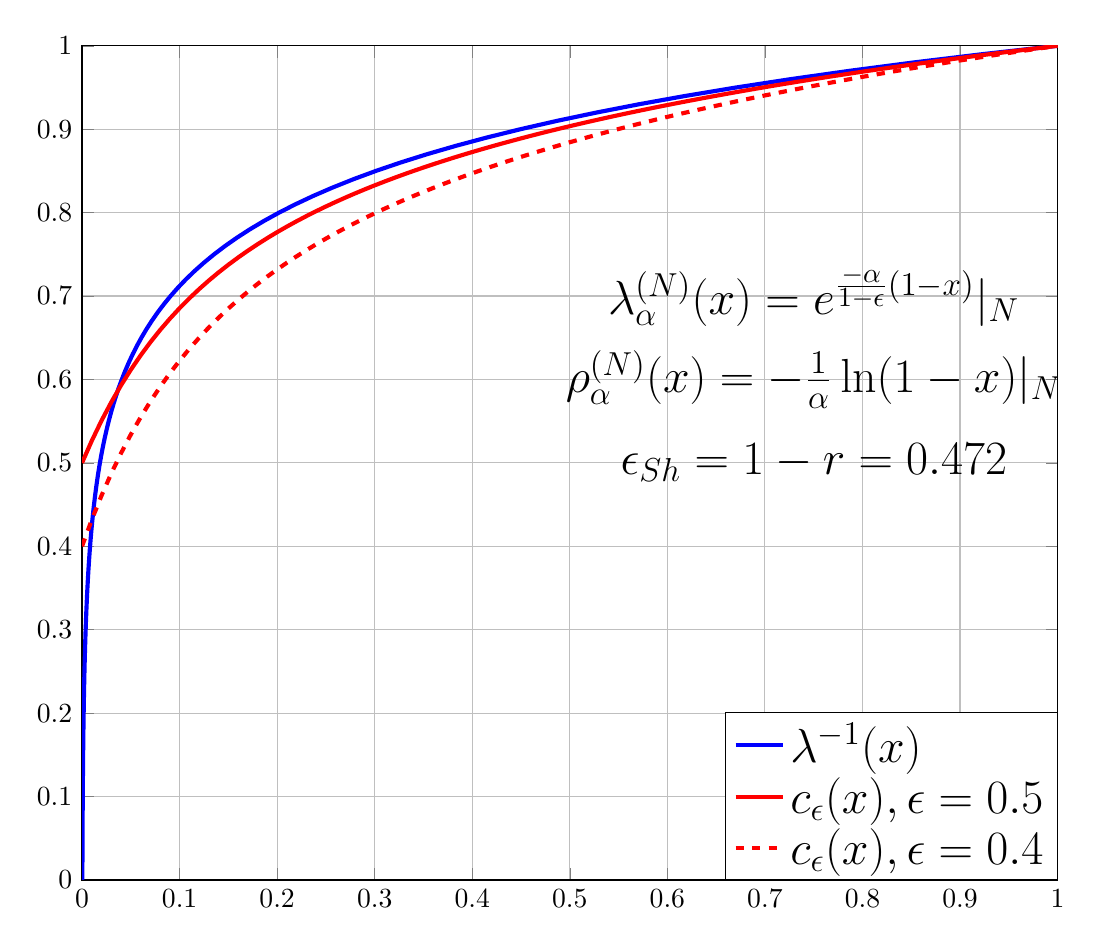
\begin{tikzpicture}
\def\fsize{\LARGE}

\begin{axis}[%
width=4.87804024496938in,
height=4.17068372703412in,
scale only axis,
xmin=0,
xmax=1,
xmajorgrids,
xtick={0,0.1,0.2,...,1},
xticklabels={0,0.1,0.2,0.3,0.4,0.5,0.6,0.7,0.8,0.9,1},
ymin=0,
ymax=1,
legend style={at={(1,0)},anchor=south east,draw=black,fill=white,legend cell align=left,font=\LARGE},
ymajorgrids
]
\node at (axis cs:0.75,0.7){\fsize{$\lambda_{\alpha}^{(N)}(x)=e^{\frac{-\alpha}{1-\epsilon} (1-x)}|_{N}$}};
%\sum\limits_{i=1}^{N}\frac{1}{\alpha}\frac{x^i}{i}}};
\node at (axis cs:0.75,0.6){\fsize{$\rho_{\alpha}^{(N)}(x)=-\frac{1}{\alpha}\ln (1-x)|_{N}$}};
%x^{\frac{1}{\alpha}},\alpha=0.1,N=50$}};
\node at (axis cs:0.75,0.5){\fsize{$\epsilon_{\text{Sh}}=1-r=0.472$}};

\addlegendentry{$\lambda^{-1}(x)$};
\addplot [color=blue,solid,line width=1.5pt]
  table[row sep=crcr]{0.000335494153584825	0\\
0.000363436477858997	0.01\\
0.000393706036385988	0.02\\
0.000426496657682508	0.03\\
0.000462018313674054	0.04\\
0.000500498464232096	0.05\\
0.000542183513693807	0.06\\
0.00058734038869107	0.07\\
0.000636258247392219	0.08\\
0.000689250331101526	0.09\\
0.000746655970072966	0.1\\
0.000808842756382345	0.11\\
0.000876208897771561	0.12\\
0.000949185767537662	0.13\\
0.00102824066679468	0.14\\
0.00111387981679615	0.15\\
0.00120665160047942	0.16\\
0.00130715007398865	0.17\\
0.00141601877066227	0.18\\
0.00153395482184343	0.19\\
0.00166171342090063	0.2\\
0.00180011265904357	0.21\\
0.00195003876389988	0.22\\
0.0021124517743976	0.23\\
0.00228839168829194	0.24\\
0.00247898512170151	0.25\\
0.00268545252329786	0.26\\
0.00290911598934362	0.27\\
0.00315140772962231	0.28\\
0.00341387923847058	0.29\\
0.00369821122963888	0.3\\
0.00400622439859745	0.31\\
0.00433989108120327	0.32\\
0.00470134788338308	0.33\\
0.00509290936270569	0.34\\
0.00551708284945217	0.35\\
0.00597658450208934	0.36\\
0.00647435669995645	0.37\\
0.00701358688453719	0.38\\
0.00759772796996556	0.39\\
0.00823052045346203	0.4\\
0.00891601636728181	0.41\\
0.00965860522554881	0.42\\
0.0104630421321226	0.43\\
0.0113344782294832	0.44\\
0.0122784936836085	0.45\\
0.0133011334160577	0.46\\
0.0144089458120634	0.47\\
0.0156090246524914	0.48\\
0.0169090545381691	0.49\\
0.0183173600974417	0.5\\
0.0198429592920402	0.51\\
0.0214956211625829	0.52\\
0.0232859283834527	0.53\\
0.0252253450275842	0.54\\
0.0273262899750436	0.55\\
0.0296022164354101	0.56\\
0.0320676980931018	0.57\\
0.0347385224271733	0.58\\
0.0376317918030286	0.59\\
0.0407660329832215	0.6\\
0.0441613157583836	0.61\\
0.0478393814576613	0.62\\
0.0518237821612379	0.63\\
0.0561400315059548	0.64\\
0.060815768049174	0.65\\
0.0658809322363014	0.66\\
0.0713679581043317	0.67\\
0.0773119809479292	0.68\\
0.0837510622765184	0.69\\
0.0907264335012647	0.7\\
0.098282759910384	0.71\\
0.106468426620664	0.72\\
0.115335848333247	0.73\\
0.124941804873458	0.74\\
0.135347804658769	0.75\\
0.146620478416798	0.76\\
0.15883200566779	0.77\\
0.172060576694392	0.78\\
0.186390892947055	0.79\\
0.201914709077521	0.8\\
0.218731420056951	0.81\\
0.23694869712112	0.82\\
0.256683176594334	0.83\\
0.278061205978336	0.84\\
0.301219652054399	0.85\\
0.326306776138336	0.86\\
0.353483182051611	0.87\\
0.382922842829663	0.88\\
0.41481421268376	0.89\\
0.449361431268097	0.9\\
0.486785627882633	0.91\\
0.527326333867846	0.92\\
0.571243012123746	0.93\\
0.618816713416241	0.94\\
0.670351869923472	0.95\\
0.726178237327734	0.96\\
0.786652997679963	0.97\\
0.852163036258837	0.98\\
0.923127406721123	0.99\\
1	1\\
};

\addlegendentry{$c_{\epsilon}(x),\epsilon=0.5$};
\addplot [color=red,solid,line width=1.5pt]
  table[row sep=crcr]{0	0.5\\
0.01	0.526526126042806\\
0.02	0.550706243040251\\
0.03	0.57280262188789\\
0.04	0.593046195873519\\
0.05	0.6116403489369\\
0.06	0.628764252863599\\
0.07	0.644575805441883\\
0.08	0.659214215869252\\
0.09	0.672802278552915\\
0.1	0.685448371847462\\
0.11	0.697248214159826\\
0.12	0.708286406177705\\
0.13	0.718637784699063\\
0.14	0.728368610616949\\
0.15	0.73753761100972\\
0.16	0.746196892968877\\
0.17	0.754392744735548\\
0.18	0.762166337885451\\
0.19	0.769554342676617\\
0.2	0.776589467232609\\
0.21	0.783300929956643\\
0.22	0.789714873441285\\
0.23	0.795854727138328\\
0.24	0.801741525169708\\
0.25	0.807394184880162\\
0.26	0.812829751044085\\
0.27	0.818063610032608\\
0.28	0.82310967771285\\
0.29	0.827980564381521\\
0.3	0.832687719622072\\
0.31	0.837241559611941\\
0.32	0.841651579088144\\
0.33	0.84592644990045\\
0.34	0.850074107836845\\
0.35	0.854101829192009\\
0.36	0.858016298362217\\
0.37	0.861823667586471\\
0.38	0.865529609810601\\
0.39	0.869139365526266\\
0.4	0.87265778432787\\
0.41	0.876089361835362\\
0.42	0.879438272548156\\
0.43	0.882708399123219\\
0.44	0.885903358507587\\
0.45	0.889026525300862\\
0.46	0.892081052675632\\
0.47	0.89506989114236\\
0.48	0.897995805409208\\
0.49	0.900861389555933\\
0.5	0.903669080713676\\
0.51	0.906421171418762\\
0.52	0.909119820787906\\
0.53	0.911767064644275\\
0.54	0.914364824708154\\
0.55	0.91691491695232\\
0.56	0.919419059210307\\
0.57	0.921878878115366\\
0.58	0.924295915438839\\
0.59	0.926671633888754\\
0.6	0.929007422422485\\
0.61	0.931304601121274\\
0.62	0.93356442566907\\
0.63	0.935788091473473\\
0.64	0.937976737462459\\
0.65	0.94013144958696\\
0.66	0.94225326405617\\
0.67	0.944343170329661\\
0.68	0.946402113887892\\
0.69	0.948430998800506\\
0.7	0.950430690109856\\
0.71	0.952402016045493\\
0.72	0.954345770083781\\
0.73	0.95626271286546\\
0.74	0.958153573982763\\
0.75	0.960019053646566\\
0.76	0.961859824243142\\
0.77	0.963676531789142\\
0.78	0.965469797292704\\
0.79	0.967240218027864\\
0.8	0.968988368728802\\
0.81	0.970714802709912\\
0.82	0.972420052917143\\
0.83	0.974104632915626\\
0.84	0.97576903781815\\
0.85	0.977413745158703\\
0.86	0.979039215714913\\
0.87	0.980645894282958\\
0.88	0.982234210408185\\
0.89	0.983804579074453\\
0.9	0.985357401354956\\
0.91	0.986893065027096\\
0.92	0.988411945153746\\
0.93	0.989914404633095\\
0.94	0.991400794719091\\
0.95	0.992871455514339\\
0.96	0.994326716437194\\
0.97	0.995766896664656\\
0.98	0.997192305552543\\
0.99	0.998603243034339\\
1	1\\
};

\addlegendentry{$c_{\epsilon}(x),\epsilon=0.4$};
\addplot [color=red,dashed,line width=1.5pt]
  table[row sep=crcr]{0	0.4\\
0.01	0.431831351251367\\
0.02	0.460847491648301\\
0.03	0.487363146265468\\
0.04	0.511655435048223\\
0.05	0.533968418724279\\
0.06	0.554517103436319\\
0.07	0.57349096653026\\
0.08	0.591057059043103\\
0.09	0.607362734263498\\
0.1	0.622538046216955\\
0.11	0.63669785699179\\
0.12	0.649943687413245\\
0.13	0.662365341638875\\
0.14	0.674042332740338\\
0.15	0.685045133211665\\
0.16	0.695436271562653\\
0.17	0.705271293682658\\
0.18	0.714599605462541\\
0.19	0.723465211211941\\
0.2	0.731907360679131\\
0.21	0.739961115947971\\
0.22	0.747657848129542\\
0.23	0.755025672565993\\
0.24	0.76208983020365\\
0.25	0.768873021856194\\
0.26	0.775395701252902\\
0.27	0.781676332039129\\
0.28	0.78773161325542\\
0.29	0.793576677257825\\
0.3	0.799225263546487\\
0.31	0.804689871534329\\
0.32	0.809981894905773\\
0.33	0.81511173988054\\
0.34	0.820088929404215\\
0.35	0.82492219503041\\
0.36	0.82961955803466\\
0.37	0.834188401103766\\
0.38	0.838635531772721\\
0.39	0.84296723863152\\
0.4	0.847189341193444\\
0.41	0.851307234202435\\
0.42	0.855325927057787\\
0.43	0.859250078947862\\
0.44	0.863084030209105\\
0.45	0.866831830361034\\
0.46	0.870497263210758\\
0.47	0.874083869370832\\
0.48	0.87759496649105\\
0.49	0.881033667467119\\
0.5	0.884402896856411\\
0.51	0.887705405702515\\
0.52	0.890943784945487\\
0.53	0.89412047757313\\
0.54	0.897237789649784\\
0.55	0.900297900342784\\
0.56	0.903302871052369\\
0.57	0.906254653738439\\
0.58	0.909155098526607\\
0.59	0.912005960666505\\
0.6	0.914808906906982\\
0.61	0.917565521345529\\
0.62	0.920277310802884\\
0.63	0.922945709768168\\
0.64	0.925572084954951\\
0.65	0.928157739504352\\
0.66	0.930703916867404\\
0.67	0.933211804395593\\
0.68	0.935682536665471\\
0.69	0.938117198560607\\
0.7	0.940516828131827\\
0.71	0.942882419254591\\
0.72	0.945214924100537\\
0.73	0.947515255438552\\
0.74	0.949784288779315\\
0.75	0.952022864375879\\
0.76	0.954231789091771\\
0.77	0.95641183814697\\
0.78	0.958563756751245\\
0.79	0.960688261633437\\
0.8	0.962786042474563\\
0.81	0.964857763251894\\
0.82	0.966904063500572\\
0.83	0.968925559498751\\
0.84	0.970922845381781\\
0.85	0.972896494190444\\
0.86	0.974847058857895\\
0.87	0.976775073139549\\
0.88	0.978681052489822\\
0.89	0.980565494889343\\
0.9	0.982428881625947\\
0.91	0.984271678032515\\
0.92	0.986094334184495\\
0.93	0.987897285559714\\
0.94	0.98968095366291\\
0.95	0.991445746617207\\
0.96	0.993192059724633\\
0.97	0.994920275997587\\
0.98	0.996630766663051\\
0.99	0.998323891641207\\
1	1\\
};
\end{axis}
\end{tikzpicture}}
  %\includegraphics[width=2.2in]{./Figures/EXIT_PoissSoliton}
\end{center}
\column{0.45\textwidth}
\begin{center}
  \includegraphics[width=2.2in]{./Figures/ratelesserasures3}
\end{center}
\end{columns}
%\begin{block}{Poisson, Soliton pair is optimal - $\lambda(x) = e^{-r_{avg}(1-x)}$}
\begin{itemize}
%\item Poisson, soliton pair is optimal
  %\item Left degree is Poisson : $\lambda(x) = e^{-r_{avg}(1-x)}$
  \item   $x = \lambda(1-(1-\epsilon)\rho(1-x))$
  \item $\lambda(x) = e^{-\frac{\alpha}{1-\epsilon}(1-x)}$, \alert{optimal right degree is soliton: $\rho(x) = -\frac{1}{\alpha}\ln(1-x)$}
  %\item \alert{Optimal distribution is soliton: $f_D[i] = \frac{1}{i(i-1)}$}
\end{itemize}
\begin{center}
\begin{tabular}{|l|c|c|c|c|c|c|c|c|}
\hline
Degree of nodes & 1 & 2 & 3 & 4 & $\ldots$ & $i$ & \ldots & $K$ \\
\hline
Fraction: \alert{ $f_D[i]$ } & $\frac{1}{K}$ & $\frac12$ & $\frac16$ & $\frac{1}{12}$ & $\ldots$ & $\frac{1}{i(i-1)}$ & \ldots & $\frac{1}{K (K-1)}$ \\
\hline
\end{tabular}
\end{center}
%\end{block}
\end{frame}
%------------------------------------------------------------------------------------
\begin{frame}{Connection with Luby Transform (LT) codes}
%\begin{columns}
%\begin{column}{0.47\textwidth}
%\begin{center}
%\includegraphics[width=1.5in]{../../Projects/MACcollision/Figures/poissonapproxerasures}
%\end{center}
%\end{column}
%\begin{column}{0.47\textwidth}
%\begin{center}
%\includegraphics[width=2.0in]{../../Projects/MACcollision/Figures/ratelesserasures}
%\end{center}
%\end{column}
%\end{columns}
\begin{center}
\includegraphics[width=3.8in]{./Figures/ratelessmaccomparison}
\end{center}
\begin{itemize}
  \item For rateless codes $\lambda(x)$ is Poisson and $\rho(x)$ is soliton
  \item For multiple access $\rho(x)$ is Poisson, \alert{optimal $\lambda(x)$ is soliton}
  \item Our result shows that both are optimal pairs
\end{itemize}
\end{frame}
%%--------------------------------------------------------------------------------------
%\begin{frame}{Histogram of required $N$ for $K=10000$}
%\begin{center}
%  \includegraphics[width=4.2in]{./Figures/fountaincodes10000histogram}
%\end{center}
%\begin{block}{Finite length considerations}
%\begin{itemize}
%  \item Deg. dist. must be adjusted for optimizing finite length performance
%  \item Raptor codes (Shokrollahi'06) is an excellent choice
%\end{itemize}
%\end{block}
%\end{frame}
%------------------------------------------------------------------------------------
%\begin{frame}{Asymptotic decoding analysis}
%\begin{itemize}
%\item Analyze the ensemble $\mathcal{G}(K,M,\lambda,\rho)$ in the limit as $K,M \rightarrow \infty$
%\item ${\sf x}_\ell$ - prob. outgoing msg from var node is erased ($\ell$-th iteration)
%\item ${\sf y}_\ell$ - prob. outgoing msg from check node is erased ($\ell$-th iteration)
%\end{itemize}
%\begin{center}
%\includegraphics[width=4.0in]{../Figures/graphicalmodelDE}
%\end{center}
%\end{frame}
%%------------------------------------------------------------------------------------
%\begin{frame}{Decoding analysis - Density evolution}
%\begin{columns}
%\begin{column}{0.4\textwidth}
%\begin{center}
%\includegraphics[width=1.6in]{../Figures/leftnode}
%\end{center}
%\small
%\begin{eqnarray}
%\nonumber x_{l,i} & = & y_l^{i-1} \\
%\nonumber x_l & = & \sum_i \lambda_i y_l^{i-1} = \lambda(y_l)
%\end{eqnarray}
%\end{column}
%\pause
%\begin{column}{0.57\textwidth}
%\begin{center}
%\includegraphics[width=1.6in]{../Figures/rightnode}
%\end{center}
%\small
%\begin{eqnarray}
%\nonumber y_{l+1,j} & = & 1-(1-x_l)^{j-1} \\
%\nonumber y_{l+1} & = & \sum_j \rho_j (1-(1-x_l)^{j-1}) = 1 - \rho(1-x_l)
%\end{eqnarray}
%\end{column}
%\end{columns}
%\end{frame}
%------------------------------------------------------------------------------------
%\normalsize
%\begin{frame}{Density evolution and successful decoding}
%\begin{columns}
%\begin{column}{0.47\textwidth}
%\begin{center}
%\includegraphics[width=1.0in]{../Figures/leftnode}
%\end{center}
%\end{column}
%\pause
%\begin{column}{0.47\textwidth}
%\begin{center}
%\includegraphics[width=1.0in]{../Figures/rightnode}
%\end{center}
%\end{column}
%\end{columns}
%\begin{block}{Density evolution}
%\vspace{-5mm}
%\begin{align*}
%{\sf x}_0 & = 1\\
%\nonumber
%{\sf y}_{\ell+1} & = 1 - \rho(1-{\sf x}_\ell) \\
%\nonumber
%{\sf x}_\ell & = \lambda({\sf y}_{\ell}) \\
%\nonumber
%{\sf y}_{\ell+1} & =  1 - \rho \left( (1-\lambda({\sf y}_{\ell}) \right)
%\end{align*}
%\end{block}
%\pause
%\begin{block}{Successful decoding condition}
%\[
%\boxed{\rho(1-\lambda(y)) > 1-y, \ \ \ y \in (0,1-\rho(0)]}
%\]
%\end{block}
%\end{frame}
%------------------------------------------------------------------------------------
\iffalse
\begin{frame}

\begin{block}{Successful decoding}
\[
\rho(1-\lambda(y)) > 1-y, \ \ \ y \in (0,1-\rho(0)]
\]
\end{block}

\begin{block}{Stability condition}
Checking the derivative of this condition at $y=0$ gives the \emph{stability condition}, $\lambda_2 \rho'(1) \leq 1$, which is also required for convergence to 0. If the inequality is strict, then $y_\ell$ converges to 0 exponentially with iteration for sufficiently large $l$.
\end{block}

\end{frame}
\fi
%%------------------------------------------------------------------------------------
%\begin{frame}{Graphical interpretation - EXIT chart}
%\begin{center}
%\includegraphics[width=3.5in]{../Figures/DEregular1}
%\end{center}
%\end{frame}
%%------------------------------------------------------------------------------------
%\begin{frame}{Graphical interpretation - EXIT chart}
%\begin{center}
%\includegraphics[width=3.5in]{../Figures/DEregular2}
%\end{center}
%\end{frame}
%------------------------------------------------------------------------------------
%\begin{frame}{Intuition behind the main result}
%%\small
%\begin{block}{Convergence follows from $\rho(1-\lambda(y)) > 1-y$}
%\begin{align*}
%\rho(1-\lambda(y)) &= 1-y \\
%e^{-\texttt{r}_{avg} \lambda(y)} &= e^{\ln(1-y)}\\
%\Rightarrow -\texttt{r}_{avg} \lambda(y)&= \ln(1-y) = -\sum_{i=1}^{\infty} \frac{y^i}{i}\\
%\Rightarrow \texttt{r}_{avg} \sum_i \lambda_i y^i & = \sum_{i=1}^{\infty} \frac{y^i}{i}
%\end{align*}
%\end{block}
%%\begin{itemize}
%%\item Analyze numerator of $\lambda^N(x)$ using $-\ln(1-x) = \sum_{i=1}^{\infty} \frac{x^i}{i}$
%%\item For $y\in(0,1)$, $-ay + \sum_{i=1}^{N} \frac{y^i}{i} < -ay -\ln(1-y)$
%%\item $\rho^N(1-\lambda^N(y)) = e^{ay-\sum_{i=1}^N \frac{y^i}{i}} > e^{\ln(1-y)} e^{ay} > (1-y)$
%%\end{itemize}
%%\end{block}
%%\vspace{-1mm}
%\pause
%\begin{block}{}
%\begin{align*}
%\texttt{r}_{avg} \lambda_i &= \frac{1}{i}\\
%\sum_i \lambda_i & = 1 \Rightarrow \boxed{\texttt{r}_{avg} = \sum_i \frac{1}{i}, \lambda_i = \frac{1/i}{\sum_i 1/i}} \Rightarrow \boxed{L_i = \frac{1}{i(i-1)}, i\geq2}
%\end{align*}
%\end{block}
%\end{frame}
%%-------------------------------------------------------------------------------------
%\begin{frame}{Precise proof}
%\begin{block}{Truncate and adjust}
%\begin{itemize}
%\item Consider $\lambda^N(x) =  \frac{L'^N(x)}{L'^N(1)} = \frac{\sum_{i=1}^{N}\frac{x^i}{i}-ax}{H(N)-a}, \ \ \rho(x) = e^{-(H(N)-a)(1-x)}$
%\item $H(N) = \sum_{i=1}^N \frac{1}{i}$
%\end{itemize}
%\end{block}
%\begin{block}{Efficiency}
%\vspace{-6mm}
%\begin{align*}
%\eta^N & = \frac{R'^N(1)}{L'^N(1)} = \frac{H(N)-a}{\frac{H(N)-a}{\sum_{i=2}^{N+1} \frac{1}{i(i-1)}-a}}
%\nonumber
%= \sum_{i=1}^{N} \frac{1}{i(i+1)}  - a = \frac{N}{N+1} - a
%\end{align*}
%\end{block}
%
%\pause
%\vspace{-6mm}
%\begin{block}{Stability}
%\begin{itemize}
%\item Expand $1-\rho(1-\lambda({\sf y}_\ell))$ around $\sf{y}_\ell = 0$ to get \vspace*{-2mm}
%\[ {\sf y}_{\ell+1} = \lambda_2^N \rho'^N(1) {\sf y}_\ell + O({\sf y}^2_\ell) = (1-a)  {\sf y}_\ell + O({\sf y}^2_\ell) \]
%%\item For any $a >  0$, the stability condition is satisfied
%\end{itemize}
%\end{block}
%\end{frame}
%---------------------------------------------------------------------------------------------------
%\begin{frame}{Precise result}
%\vspace{-4mm}
%%\begin{itemize}
%%\item Soliton distribution,  $L(x) = \sum_{i=2}^{\infty} \frac{x^i}{i(i-1)}$, is optimal
%%\end{itemize}
%%\pause
% \begin{block}{}
% {Theorem: For any $a\in[0,1]$, consider the sequence (indexed by $N\in \mathbb{N}$) of node-perspective degree-distributions,  $(L^N(x),R^N(x))$, where
%\begin{align*}
%L^N(x) &= \frac{\sum_{i=2}^{N+1}\frac{x^i}{i(i-1)}-\frac{a x^2}{2}}{\sum_{i=2}^{N+1}\frac{1}{i(i-1)}-\frac{a}{2}} \\
%R^N(x) &= e^{-\left(H(N)-a\right)(1-x)}.
%\end{align*}
%Here $H(N) = \sum_{i=1}^N \frac{1}{i}$ is the $N$-th Harmonic number. For every ensemble in this sequence, ${\sf y}_\ell \stackrel{\ell \rightarrow \infty}{\rightarrow} 0$ while $\eta^N = \frac{N}{N+1} - a \stackrel{N \rightarrow \infty}{\rightarrow} 1-a$.}
%\end{block}
%%\vspace{2mm}
%%\alert{Stability:} For any $a>0$, the stability condition is strictly satisfied
%
%\begin{block}{}
%For $\eta \rightarrow 1$, $\texttt{r}_{avg} \rightarrow \infty \Rightarrow P$(right degree $=1) \rightarrow 0$
%\end{block}
%\end{frame}
%------------------------------------------------------------------------------------
\begin{frame}{Simulation Results}
\begin{center}
\includegraphics[width=3.2in]{C:/Users/nrkri/Dropbox/Work/RESEARCH/Projects/MACcollision/Figures/Simulationresultserasure}
\end{center}
\begin{itemize}
\item Even for $K=10000$, efficiency close to 0.8 can be obtained
\end{itemize}
\end{frame}
%------------------------------------------------------------------------------------
\begin{frame}{Some open problems}
\begin{itemize}
\item Fundamental limits on universal multiple access, i.e. $K$, $\epsilon$ not known
\item Uncoordinated multiple access with power constraint and Gaussian noise
    \begin{itemize}
    \item Power penalty for repeating information $\log n$ times on the average
    \item Can we achieve the equal rate point on the MAC region with simple decoding?
    \end{itemize}
\end{itemize}
\end{frame}
%------------------------------------------------------------------------------------
%\begin{frame}{Average Degree and its Consequences}
%\begin{block}{Optimal distribution is soliton: $f(i) = \frac{1}{i(i-1)}$}
%\begin{center}
%\begin{tabular}{|l|c|c|c|c|c|c|}
%\hline
%No. of times & 1 & 2 & 3 & 4 & $\ldots$ & $M$ \\
%\hline
%Fraction of users & 0 & $\frac12$ & $\frac16$ & $\frac{1}{12}$ & $\ldots$ & $\frac{1}{M (M-1)}$ \\
%\hline
%\end{tabular}
%\end{center}
%\end{block}
%\begin{block}{Average degree}
%\begin{itemize}
%\item Average left degree is $\ln M \Rightarrow $ average right degree is $\eta \ln M$
%\item For $K,M \rightarrow \infty$, $\texttt{r}_{avg} \rightarrow \infty \Rightarrow P$(right degree $=1) \rightarrow 0$
%\end{itemize}
%\end{block}
%\pause
%\begin{block}{Consequences}
%\begin{itemize}
%\item Consequence 1: Iterations can get stuck at the beginning
%\item Consequence 2: Average power consumed is $\ln K$ times larger
%\item Data is not centrally available - joint precoding is not an option
%\end{itemize}
%\end{block}
%\end{frame}
%\begin{frame}{Non-Asymptotic Regime - Non-Poisson Right degrees?}
%%\vspace{-2mm}
%\begin{itemize}
%\item For fixed number of users $K$, is this scheme still the optimal thing to do?
%\item<2-> Each user picks the time-slots uniformly at random (uniform PMF)
%\item<2-> What about other PMFs?
%\item<2-> By picking step like PMF, we can induce mixture of Poisson distributions
%\end{itemize}
%\pause
%\begin{figure}
%\input{../Figures/PMFs_Uniform_Steplike.tex}
%\end{figure}
%\end{frame}

%\begin{frame}{Simulation Results, $K = 1000$}
%\begin{figure}
%\input{../../Projects/MACcollision/Figures/BERvsEfficiency.tex}
%\end{figure}
%\end{frame}

%\begin{frame}{Analysis of Peeling Decoder}
%\begin{itemize}
%\item Uniform leads to $\rho(x)$ =Poisson distribution, step-like PMF results in mixture of two Poisson PMFs.
%\item $\rho_{1}$ for Poisson mixture is higher thus a lower probability of peeling decoder getting stuck in the initial stages.
%\end{itemize}
%\begin{figure}
%\input{../Figures/ResidualGraph_Degree1Nodes.tex}
%\caption{Expected path in the residual graph of peeling decoder}
%\end{figure}
%\end{frame}
